\section{随机采样与积分计算}
\label{sec:dtsp-sampling}

本节把前面的工具用于一个计算任务：近似一个固定的积分
\[
  I=\int_Ef\,\mathrm d\pi=\mathbb E_\pi f(X).
\]
被积分布$\pi$可能只知道到一个归一化常数为止，例如给定一组已经观测到的数据后，参数的后验密度正比于“先验密度乘以似然”，而比例常数本身就是一个难算的积分。思路是生成一列随机样本，使它们的平均接近$I$。样本可以相互独立，也可以来自一条以$\pi$为不变分布的Markov链；无论状态是实数还是向量，样本按编号排成的都是离散时间随机序列。我们依次讨论样本怎样生成、各样本的贡献怎样加权、误差怎样评估。这里研究的是数值计算误差：$I$作为统计量有什么含义、怎样从数据推断，由统计推断部分说明。

\subsection{独立采样与样本平均}
\label{sec:dtsp-iid-sampling}

\paragraph{从均匀随机数到指定分布}
计算机能直接产生的是$(0,1)$上的均匀随机数（更准确地说，是通过统计检验的伪随机数）。其他分布都要由它变换而来。最直接的变换是把累积分布函数“倒过来用”。对实值分布函数$F$，定义广义逆$F^{-1}(u)=\inf\{x:F(x)\geq u\}$。

\begin{theorem}[逆变换采样]
  \label{thm:dtsp-inverse-transform}
  若$U\sim\operatorname{Unif}(0,1)$，则$X=F^{-1}(U)$的分布函数为$F$。
\end{theorem}

\begin{proof}
$F$右连续且单调不减，所以$\{x:F(x)\geq u\}$是一个包含左端点的区间$[F^{-1}(u),\infty)$。于是$F^{-1}(u)\leq x$当且仅当$u\leq F(x)$，从而$\mathbb P(X\leq x)=\mathbb P(U\leq F(x))=F(x)$。
\end{proof}

图~\ref{fig:dtsp-inverse-rejection}(a)用指数分布演示这一步：在纵轴上取均匀数$u$，水平走到曲线$F(x)=1-e^{-x}$，再竖直落到横轴，得到$x=-\log(1-u)$。曲线陡的地方，纵轴上的一小段对应横轴上的一小段，样本密集；曲线平的地方样本稀疏，正好对应密度的高低。离散分布同样适用：把概率依次累加，看$u$落在哪一段。这个方法要求能够计算$F^{-1}$，多维分布一般做不到。

\paragraph{拒绝采样}
若只能计算目标密度$p$（甚至只知道它的常数倍），却能从另一个密度$g$采样，且$p\leq Mg$对某个常数$M$成立，可以“先多抽，再筛掉”。把$Mg$的图像想成罩在$p$外面的帐篷：在帐篷下均匀撒点，只保留落在$p$曲线下方的点，这些点的横坐标就服从$p$。具体步骤是：抽取$Y\sim g$与独立的$U\sim\operatorname{Unif}(0,1)$；若$U\leq p(Y)/(Mg(Y))$则输出$Y$，否则重来。

\begin{theorem}[拒绝采样]
  \label{thm:dtsp-rejection}
  在上述条件下，每轮被接受的概率为$1/M$，所需轮数服从均值为$M$的几何分布，输出的样本密度为$p$。
\end{theorem}

\begin{proof}
对可测集$B$，
\[
  \mathbb P(Y\in B,\ \text{接受})=\int_Bg(y)\frac{p(y)}{Mg(y)}\,\mathrm dy=\frac1M\int_Bp(y)\,\mathrm dy.
\]
取$B$为全空间得接受概率$1/M$；两式相除得到接受条件下$Y$的分布为$p$。各轮独立，所以轮数服从几何分布。
\end{proof}

若只知道$\tilde p=Zp$且$\tilde p\leq\tilde Mg$，算法照样执行，接受概率变为$Z/\tilde M$，未知常数$Z$不需要算出。图~\ref{fig:dtsp-inverse-rejection}(b)从均匀分布中为密度$6x(1-x)$采样，帐篷高度取其最大值$M=1.5$，理论接受率为$2/3$；图中$260$个候选点接受了$167$个。拒绝采样的代价在高维中急剧上升。用$d$维立方体$[-1,1]^d$罩住单位球、在球内均匀采样，接受率是体积比$\pi^{d/2}/(\Gamma(d/2+1)2^d)$：$d=2$时为$0.785$，$d=10$时只有约$0.0025$，平均要试四百次才得到一个样本。

\begin{figure}[htbp]
  \centering
  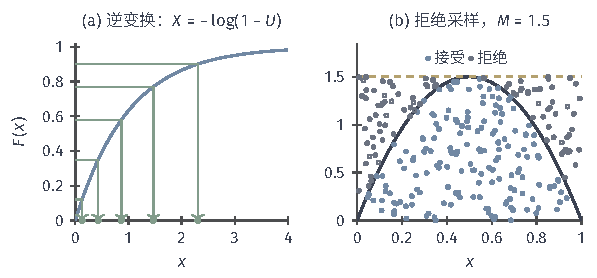
\includegraphics[width=101mm]{figures/03-optimization-evolution-and-signals/02-processes-and-trajectory-evolution/tikz/dtsp-inverse-rejection/figure.pdf}
  \caption{由均匀随机数生成样本。(a)逆变换：纵轴上的五个均匀数$u$沿绿线经指数分布函数$F(x)=1-e^{-x}$映到横轴上的样本$-\log(1-u)$；(b)拒绝采样：在高度$M=1.5$的均匀“帐篷”下撒$260$个点（固定随机种子），落在密度$6x(1-x)$下方的点（实心）被接受，其横坐标服从该密度。}
  \label{fig:dtsp-inverse-rejection}
\end{figure}

\paragraph{样本平均与Monte Carlo积分}
有了独立样本$X_1,\ldots,X_n\sim\pi$，最自然的估计是样本平均
\[
  \widehat I_n=\frac1n\sum_{i=1}^nf(X_i),
\]
称为\term{Monte Carlo积分}（Monte Carlo integration）。若$\pi(|f|)<\infty$，它无偏；若$\sigma^2=\operatorname{Var}_\pi f(X)<\infty$，则$\operatorname{Var}(\widehat I_n)=\sigma^2/n$。对它要分清三种不同的误差陈述。一致性：由强大数律，$\widehat I_n\to I$几乎必然，只需要$\pi(|f|)<\infty$。均方误差：$\mathbb E(\widehat I_n-I)^2=\sigma^2/n$是精确等式，需要$\sigma^2<\infty$。数值标准误：实际计算时$\sigma^2$未知，用样本方差$\widehat\sigma^2_n$代替，报告$\widehat\sigma_n/\sqrt n$；由中心极限定理与Slutsky定理，在$0<\sigma^2<\infty$时$\widehat I_n\pm1.96\,\widehat\sigma_n/\sqrt n$渐近地以$95\%$的概率覆盖$I$。前两条是关于估计量的性质，第三条是对误差大小的数值估计，它本身也有误差。

以$I=\int_0^1x^2\,\mathrm dx=1/3$为贯穿例子，$X\sim\operatorname{Unif}(0,1)$，$f(x)=x^2$，单样本方差$\sigma^2=\frac15-\frac19=\frac4{45}$。$n=10^4$时标准误约为$0.003$。图~\ref{fig:dtsp-monte-carlo-rate}(a)在双对数坐标上画出十二次独立运行的绝对误差，它们围绕斜率为$-1/2$的直线$\sqrt{4/(45n)}$上下起伏；(b)显示$n=400$时缩放误差$\sqrt n(\widehat I_n-I)$的直方图与$\mathcal N(0,4/45)$密度吻合。

\begin{figure}[htbp]
  \centering
  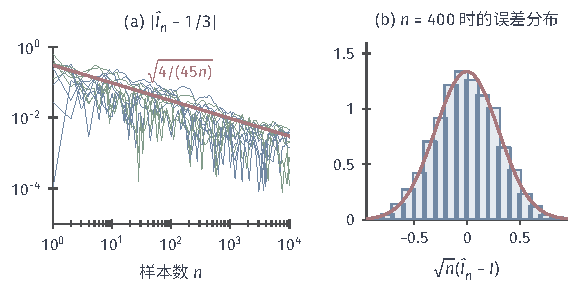
\includegraphics[width=97mm]{figures/03-optimization-evolution-and-signals/02-processes-and-trajectory-evolution/tikz/dtsp-monte-carlo-rate/figure.pdf}
  \caption{Monte Carlo积分$\int_0^1x^2\,\mathrm dx$的误差。(a)$12$次独立运行的$|\widehat I_n-1/3|$（双对数坐标），红线为均方根误差$\sqrt{4/(45n)}$；(b)$n=400$时$3000$次重复的$\sqrt n(\widehat I_n-I)$直方图，红线为$\mathcal N(0,4/45)$密度。}
  \label{fig:dtsp-monte-carlo-rate}
\end{figure}

\paragraph{维数的作用}
$n^{-1/2}$的速度与被积变量的维数$d$无关，这是Monte Carlo相对于网格求积的主要优势：网格方法在$d$维中用$n$个点，每个方向只有$n^{1/d}$个点，精度随$d$急剧下降。但“与维数无关”只针对指数，不针对常数。设$X$在$[0,1]^d$上均匀，估计$p=\mathbb P(\text{所有坐标}\leq0.9)=0.9^d$。单样本相对标准差是$\sqrt{(1-p)/p}$；$d=50$时$p\approx0.0052$，相对标准差约$13.9$，要把相对误差压到$1\%$需要约$1.9\times10^6$个样本。维数通过方差$\sigma^2$和每个样本的生成成本进入计算量。下面两小节的方法都着眼于在不改变$I$的前提下减小$\sigma^2$。

\subsection{重要性抽样与自归一化}
\label{sec:dtsp-importance}

\paragraph{换一个分布来抽样}
上面的例子中，大部分样本落在对积分毫无贡献的区域。若改从另一个分布$q$抽样，让样本更多地落在$|f|p$大的地方，再给每个样本乘一个修正权重，就可能在保持期望的同时降低方差。设$\pi$与$q$关于同一参考测度分别有密度$p,q$，并且
\begin{equation}
  q(x)>0\quad\text{在}\ \{x:f(x)p(x)\neq0\}\ \text{上几乎处处成立}.
  \label{eq:dtsp-is-support}
\end{equation}
记$w=p/q$（在$q>0$处定义），则$I=\int fp=\int(fw)q=\mathbb E_q[f(X)w(X)]$。当$\pi\ll q$时，$w$就是Radon--Nikodym导数$\mathrm d\pi/\mathrm dq$，换测度公式可参考\BookChapterRef{chap:densities-change-of-measure}{卷二“密度与换测度”章}。由此得到\term{重要性抽样}（importance sampling）估计
\begin{equation}
  \widehat I_n^{\mathrm{IS}}=\frac1n\sum_{i=1}^nw(X_i)f(X_i),\qquad X_i\ \text{独立同分布于}\ q.
  \label{eq:dtsp-importance-sampling}
\end{equation}
它无偏，只要$\mathbb E_q|fw|<\infty$；其方差为$\frac1n(\mathbb E_q[f^2w^2]-I^2)$，有限二阶矩$\mathbb E_q[f^2w^2]<\infty$是一项额外要求。支撑条件~\eqref{eq:dtsp-is-support}不能省略：若$q$在$fp$有质量的区域为零，那里永远采不到样本，估计量对准的就不是$I$。

仍以$\int_0^1x^2\,\mathrm dx$为例，取$q(x)=2x$，则$w(x)=1/(2x)$，$f(x)w(x)=x/2$，单样本方差为$\mathbb E_q[X^2/4]-\frac19=\frac18-\frac19=\frac1{72}$，比直接平均的$4/45$小六倍多。这次改进来自$q$把样本更多地放在$x^2$大的地方。

\paragraph{最优提议与重尾风险}
什么样的$q$最好？由Cauchy--Schwarz不等式，在满足条件~\eqref{eq:dtsp-is-support}的密度中，
\[
  \Bigl(\int|f|p\Bigr)^2=\Bigl(\int_{\{q>0\}}\frac{|f|p}{\sqrt q}\sqrt q\Bigr)^2\leq\int\frac{f^2p^2}{q}=\mathbb E_q[f^2w^2],
\]
等号当且仅当$q\propto|f|p$。所以二阶矩最小的提议是$q^\star=|f|p/\int|f|p$；若$f\geq0$，此时$fw\equiv I$，方差为零。这个理想提议通常不能直接使用，因为它的归一化常数就是要算的积分；但它指明了方向：提议应当在$|f|p$大的地方有足够的质量，尾部不能比$|f|p$轻。

尾部过轻的后果可以精确算出。取目标$p=\mathcal N(0,1)$、$f\equiv1$，提议$q=\mathcal N(0,s^2)$，则$w(x)=s\exp\bigl(x^2(s^{-2}-1)/2\bigr)$，
\[
  \mathbb E_qw^2=\int\frac{p^2}{q}=\frac{s^2}{\sqrt{2s^2-1}}\qquad(s^2>1/2),
\]
而$s^2\leq1/2$时积分发散。图~\ref{fig:dtsp-importance-variance}(a)画出这条曲线：$s=1$时为$1$，偏离$1$时增大，越过$1/\sqrt2$后变为无穷。方差无穷时估计量仍然无偏、仍然几乎必然收敛，但它的误差不再按$n^{-1/2}$规律下降，常常表现为长时间平稳后被一个巨大权重突然推开；图(b)中$s=0.6$的运行在前几十个样本内就出现了这样的跳跃，而$s=1.6$的运行平稳得多。

\begin{figure}[htbp]
  \centering
  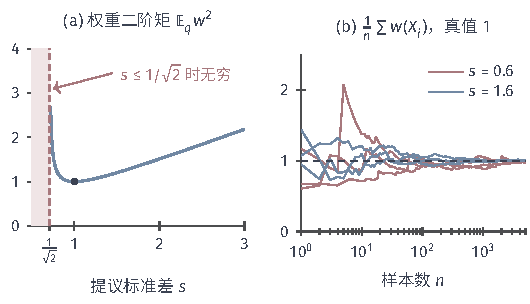
\includegraphics[width=90mm]{figures/03-optimization-evolution-and-signals/02-processes-and-trajectory-evolution/tikz/dtsp-importance-variance/figure.pdf}
  \caption{提议尾部与重要性权重的方差。目标为$\mathcal N(0,1)$，提议为$\mathcal N(0,s^2)$，权重$w=p/q$，估计对象为$\mathbb E_qw=1$。(a)精确的二阶矩$\mathbb E_qw^2=s^2/\sqrt{2s^2-1}$，在$s\leq1/\sqrt2$（阴影）时为无穷；(b)$s=0.6$与$s=1.6$各三次运行的累计平均（横轴对数刻度，固定随机种子）。}
  \label{fig:dtsp-importance-variance}
\end{figure}

反过来，选得好的提议可以把方差降低几个数量级。估计罕见事件概率$p_4=\mathbb P(Z>4)\approx3.17\times10^{-5}$，$Z\sim\mathcal N(0,1)$。直接平均示性函数时，单样本相对方差为$(1-p_4)/p_4\approx3.2\times10^4$。改从$\mathcal N(4,1)$抽样，权重为$e^{-4x+8}$，二阶矩为
\[
  \int_4^\infty\varphi(x)e^{-4x+8}\,\mathrm dx=e^{16}\int_4^\infty\varphi(x+4)\,\mathrm dx=e^{16}\,\mathbb P(Z>8)\approx5.5\times10^{-9},
\]
其中$\varphi$是标准正态密度。相对方差降为$5.5\times10^{-9}/p_4^2-1\approx4.5$。同样的精度所需样本数缩小约七千倍。

\paragraph{只知道未归一化密度}
很多目标只知道$\tilde p=Zp$，常数$Z$未知，于是权重$w$也只知道常数倍$\tilde w=\tilde p/q=Zw$。把加权和除以权重和，未知常数就约掉了：
\begin{equation}
  \widehat I_n^{\mathrm{SN}}=\frac{\sum_{i=1}^n\tilde w(X_i)f(X_i)}{\sum_{i=1}^n\tilde w(X_i)}.
  \label{eq:dtsp-self-normalized-is}
\end{equation}
这称为自归一化重要性抽样。若$\mathbb E_q|f\tilde w|<\infty$，强大数律给出分子$/n\to ZI$、分母$/n\to Z$几乎必然，所以$\widehat I_n^{\mathrm{SN}}\to I$几乎必然。但它是两个随机量之比，一般有偏，因为$\mathbb E[A/B]\neq\mathbb EA/\mathbb EB$；偏差的量级为$O(1/n)$。把比值在$(ZI,Z)$附近线性化，可以得到它的渐近方差约为$\frac1n\mathbb E_q[w^2(f-I)^2]$：与$f$本身相比，起作用的是中心化后的$f-I$。

自归一化之外，实践中常见的两个修补都有代价。设三点空间上$q=(0.8,0.15,0.05)$、$p=(0.4,0.3,0.3)$，则$w=(0.5,2,6)$；对$f=(0,1,1)$，$I=0.6$，单样本贡献$wf=(0,2,6)$的方差为$0.15\times4+0.05\times36-0.36=2.04$。若把权重截断在$2$，方差降到$0.64$，但均值变成$0.4$，引入了$-0.2$的偏差，截断必须连同偏差一起报告。若按归一化权重重采样，样本被复制成等权粒子，权重不均的问题在后续计算中得到缓解，却增加了额外的随机性。常用的诊断量$\widehat n_{\mathrm{eff}}=(\sum_i\tilde w_i)^2/\sum_i\tilde w_i^2$度量权重退化的程度，它不是严格意义上的独立样本数，也不能说明偏差已经消失。还应注意，这里的“自归一化”指用权重和作分母，与第~\ref{sec:dtsp-maximal-tail}节用设计矩阵归一化累计噪声不是同一个概念。

\subsection{固定积分的方差缩减}
\label{sec:dtsp-variance-reduction}

本小节的方法都保持积分目标不变，只改变样本贡献的写法或样本之间的搭配。比较时要固定同一个积分和同样的计算预算（例如被积函数的求值次数），再比较方差与额外的计算或先验信息。

\paragraph{控制变量}
若手头有一个与$f(X)$一起波动、且均值$\mu_h$已知的辅助量$h(X)$，可以减去它偏离均值的部分。对任意常数$\beta$，$f_\beta=f-\beta(h-\mu_h)$的期望仍是$I$，方差为$\operatorname{Var}f-2\beta\operatorname{Cov}(f,h)+\beta^2\operatorname{Var}h$。对$\beta$求最小，得到
\[
  \beta^\star=\frac{\operatorname{Cov}(f,h)}{\operatorname{Var}h},\qquad
  \operatorname{Var}f_{\beta^\star}=(1-\rho_{f,h}^2)\operatorname{Var}f,
\]
其中$\rho_{f,h}$是二者的相关系数：相关越强，剩下的方差越少。对$f(x)=x^2$、$h(x)=x$、$X\sim\operatorname{Unif}(0,1)$，$\mu_h=1/2$，$\operatorname{Cov}(X^2,X)=\frac14-\frac16=\frac1{12}$，$\operatorname{Var}X=\frac1{12}$，于是$\beta^\star=1$，调整后的被积量$x^2-x+\frac12$方差为$\frac1{180}$，是原来的$1/16$。实际中$\beta^\star$也要从同一批样本估计；这时估计量不再严格无偏，误差公式也要计入系数的随机性，只是大样本下这一影响是高阶的。

\paragraph{条件平均}
若估计过程中抽取了对目标不必要的额外随机量，可以把它积分掉。设$Y$是$I$的无偏估计，$\mathbb EY^2<\infty$，$T$是某个能直接计算条件期望的统计量，令$Y^\star=\mathbb E[Y\mid T]$。塔式性质给出$\mathbb EY^\star=I$，全方差公式给出
\[
  \operatorname{Var}Y=\mathbb E[\operatorname{Var}(Y\mid T)]+\operatorname{Var}Y^\star\geq\operatorname{Var}Y^\star.
\]
这称为\term{Rao--Blackwell化}（Rao--Blackwellization）。例如在单位正方形中撒点、数落在曲线$u=x^2$下方的比例（命中法）：$Y=\mathbb I\{U\leq X^2\}$，$\operatorname{Var}Y=\frac13\cdot\frac23=\frac29$。对$X$取条件期望，$\mathbb E[Y\mid X]=X^2$，正是直接平均，方差降为$4/45$。图~\ref{fig:dtsp-rao-blackwell}把条件平均解释为竖切片上命中区段的长度：给定$X=0.6$，再抽一次$U$只会得到$0$或$1$，而它的条件均值$0.36$可以直接算出。

\begin{figure*}[htbp]
  \centering
  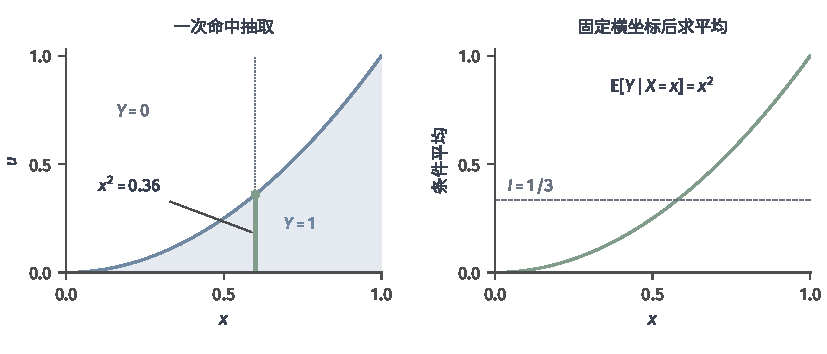
\includegraphics[width=140mm]{figures/00-shared/mathematical-preliminaries-lower/01-random-variables-distributions-and-causality/matplotlib/probability-rao-blackwell-slice/figure.pdf}
  \caption{命中积分的Rao--Blackwell化（解析式教学图）。独立的$X,U$均在$(0,1)$上均匀分布。左图阴影为$U\leq X^2$，竖切片$x=0.6$的命中长度为$0.36$；右图保留每个$x$对应的条件均值$x^2$。两个估计量的期望均为$1/3$，单样本方差分别为$2/9$与$4/45$。}
  \label{fig:dtsp-rao-blackwell}
\end{figure*}

\paragraph{对偶变量}
上面两种方法改造单个样本的贡献；另一类方法改变样本之间的搭配。若$f$单调，$X$与$1-X$给出的$f$值一大一小，把它们配成一对取平均，正负误差会部分抵消。一对的平均$\frac12(f(X)+f(1-X))$的方差为$\frac{\sigma^2}2(1+\rho)$，其中$\rho=\operatorname{Corr}(f(X),f(1-X))$；与两个独立样本的平均$\sigma^2/2$相比，$\rho<0$时有改进。对$f(x)=x^2$，一对的平均恰为$x^2-x+\frac12$，方差为$1/180$，按每次函数求值折算为$1/90$。改进依赖负相关，并非无条件成立：若$f(x)=(x-\frac12)^2$关于$\frac12$对称，则$f(X)=f(1-X)$，$\rho=1$，配对平均的方差是独立两样本的两倍。

\paragraph{分层采样}
另一种搭配方式是把样本按比例分配到各个区域。把$[0,1]$分成$K$个等长小区间，每个区间里各取$n/K$个均匀点，用各区间平均的加权和估计$I$。记第$j$层的条件方差为$\sigma_j^2$、层内均值为$\mu_j$，按比例分配时估计量的方差为$\frac1n\sum_j\frac1K\sigma_j^2$。由全方差公式，$\sigma^2=\sum_j\frac1K\sigma_j^2+\sum_j\frac1K(\mu_j-I)^2$，所以分层永远不会比直接平均差，并且去掉了层与层之间的波动。$K=10$、每层一个点时，$n\operatorname{Var}=0.0011$，在这个光滑一维例子中优于前面所有方法。分层的效果依赖于能否把空间切成层内变化小的区域；高维中层数随维数指数增长，必须改用更粗的分层或自适应分层。

图~\ref{fig:dtsp-variance-reduction}把这些方法放在同一个积分、同样的函数求值预算下比较。排序只对这一个光滑的一维积分成立：它展示的是各种方法起作用的机制与代价，不是对其他问题的普遍排名。重要性抽样需要能从$q$采样并计算密度比，控制变量需要已知的辅助均值，对偶变量需要单调性，分层需要能在每层内条件采样。

\begin{figure}[htbp]
  \centering
  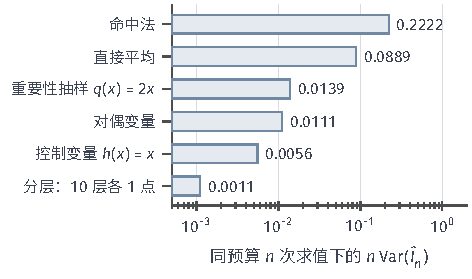
\includegraphics[width=80mm]{figures/03-optimization-evolution-and-signals/02-processes-and-trajectory-evolution/tikz/dtsp-variance-reduction/figure.pdf}
  \caption{同一积分$\int_0^1x^2\,\mathrm dx$在$n$次被积函数求值预算下的$n\operatorname{Var}(\widehat I_n)$（精确值，横轴对数刻度）。命中法为$2/9$，直接平均为$4/45$，对偶变量按每次求值折算为$1/90$，重要性抽样（$q(x)=2x$）为$1/72$，控制变量（$h(x)=x$，$\beta=1$）为$1/180$，分层为十个等长层各取一点。}
  \label{fig:dtsp-variance-reduction}
\end{figure}

\subsection{Markov链采样}
\label{sec:dtsp-mcmc}

当$\pi$的维数高、形状复杂、只知道未归一化密度$\tilde\pi$时，逆变换、拒绝采样和简单的重要性抽样往往都不可行。换一个思路：不直接从$\pi$采样，而是设计一条以$\pi$为不变分布的Markov链，让它长时间运行，再用遍历定理把时间平均当作积分。第~\ref{sec:dtsp-reversibility}节说明，细致平衡是保证不变性的便利条件，它只涉及两个状态的密度比，未知的归一化常数自然约掉。这类方法统称为\term{Markov链蒙特卡洛}（Markov chain Monte Carlo）。

\paragraph{Metropolis--Hastings}
设$\pi$关于参考测度有密度，$\tilde\pi\propto\pi$可计算；$q(x,y)$是一个可以采样的提议密度。\term{Metropolis--Hastings方法}（Metropolis--Hastings）的一步是：在当前状态$x$处抽取候选$y\sim q(x,\cdot)$，以概率
\begin{equation}
  a(x,y)=\min\Bigl\{1,\ \frac{\tilde\pi(y)q(y,x)}{\tilde\pi(x)q(x,y)}\Bigr\}
  \label{eq:dtsp-mh-acceptance}
\end{equation}
接受并移到$y$，否则停在$x$\scite{pgm-history-metropolis1953,pgm-history-hastings1970}。停在原地也要记为一个样本，否则会改变链的不变分布。所得转移核为$P(x,\mathrm dy)=q(x,y)a(x,y)\,\mathrm dy+r(x)\delta_x(\mathrm dy)$，其中$r(x)=1-\int q(x,y)a(x,y)\,\mathrm dy$是拒绝概率。

\begin{theorem}[Metropolis--Hastings的细致平衡]
  \label{thm:dtsp-mh-balance}
  上述转移核关于$\pi$满足细致平衡，因而以$\pi$为不变分布。
\end{theorem}

\begin{proof}
对$x\neq y$，由式~\eqref{eq:dtsp-mh-acceptance}，
\[
  \pi(x)q(x,y)a(x,y)=\min\{\pi(x)q(x,y),\ \pi(y)q(y,x)\},
\]
右侧关于$x,y$对称，所以两点之间的正反流量相等。拒绝部分集中在对角线$\{y=x\}$上，在交换$x,y$时本身不变。两部分合起来就是式~\eqref{eq:dtsp-detailed-balance}，再由定理~\ref{thm:dtsp-detailed-balance}得到不变性。
\end{proof}

接受率只用到密度比$\tilde\pi(y)/\tilde\pi(x)$，归一化常数不需要知道。若提议对称，$q(x,y)=q(y,x)$（例如$y=x+\varepsilon$、$\varepsilon\sim\mathcal N(\bm 0,s^2\bm I)$），接受率化为$\min\{1,\tilde\pi(y)/\tilde\pi(x)\}$：往高密度处走一定接受，往低密度处走按比例接受。每一步只需一次提议和一次$\tilde\pi$求值。

\paragraph{从不变到可用}
细致平衡只保证“从$\pi$出发会留在$\pi$”。要让任意初态出发的时间平均收敛到$I$，还要第~\ref{sec:dtsp-long-run}节的回返条件。随机游走提议的密度处处为正时，链是$\pi$不可约的；只要拒绝以正概率发生，链就是非周期的；在这些条件下Metropolis--Hastings链是正Harris常返的，遍历定理适用\scite{math-meyn2009markov}。但这些定性条件不保证收敛得快。随机游走的步长$s$是关键：步长小，几乎总被接受，但每步只挪一点，路径像扩散一样缓慢；步长大，多数提议落到低密度区而被拒绝，链经常原地不动。两种情形的自相关都很高。

图~\ref{fig:dtsp-mh-gibbs}(a)对相关系数$0.95$的二维正态目标运行随机游走Metropolis--Hastings，$s=0.35$，长程接受率约$0.56$。目标的高密度区是一条细长的斜脊，提议在各方向同样大小，所以沿脊的移动只能靠许多小步累积；(c)中第一坐标的自相关在间隔$40$处仍约为$0.5$。

\paragraph{Gibbs采样}
另一种构造利用条件分布。设$x=(x_1,\ldots,x_d)$，若能从每个满条件分布$\pi(x_j\mid x_{-j})$中直接采样，就可以每次只更新一个坐标、其余坐标不动。这就是\term{Gibbs采样}（Gibbs sampling）\scite{pgm-history-geman1984}。单坐标更新核$K_j$保持$\pi$：若$X\sim\pi$，则$X_{-j}$服从$\pi$的边缘，再从$\pi(\cdot\mid X_{-j})$抽出新的第$j$坐标，联合分布仍是$\pi$。它也可以看成提议恰为满条件分布的Metropolis--Hastings，此时式~\eqref{eq:dtsp-mh-acceptance}中的比值恒为$1$，所以每个$K_j$都满足细致平衡。

把各坐标的更新组合起来有两种方式。按固定顺序依次更新（系统扫描），一轮的核是$K_1K_2\cdots K_d$；每个因子保持$\pi$，乘积也保持$\pi$，但乘积一般不再可逆。每轮随机选一个坐标更新（随机扫描），核为$\frac1d\sum_jK_j$，仍满足细致平衡。把强相关的坐标合成一块一起更新，称为分块Gibbs，往往比逐个坐标快得多。

对相关系数为$\rho$的标准二维正态，满条件分布为$x_1\mid x_2\sim\mathcal N(\rho x_2,1-\rho^2)$，另一个对称。系统扫描一轮后，第一坐标满足$x_1'=\rho^2x_1+\eta$，$\eta$与$x_1$独立，因此它是系数为$\rho^2$的一阶递推，自相关为$\rho^{2k}$，积分自相关时间为$(1+\rho^2)/(1-\rho^2)$。$\rho=0.95$时约为$19.5$。图~\ref{fig:dtsp-mh-gibbs}(b)中Gibbs路径只能沿坐标方向横竖移动，在斜脊上走出细碎的阶梯；(c)中它的自相关与$\rho^{2k}$吻合，衰减比随机游走快，但仍远慢于独立样本。

\begin{figure*}[htbp]
  \centering
  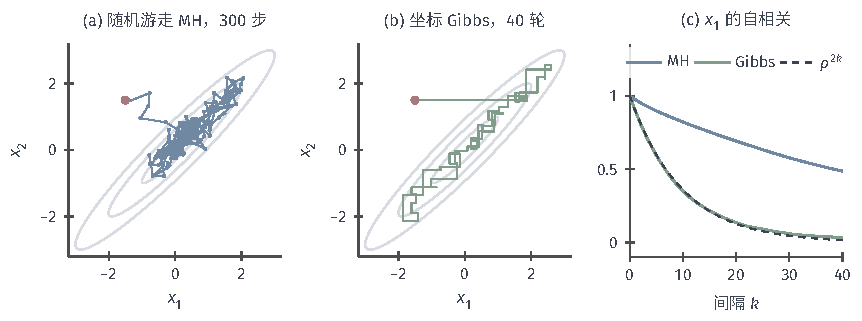
\includegraphics[width=146mm]{figures/03-optimization-evolution-and-signals/02-processes-and-trajectory-evolution/tikz/dtsp-mh-gibbs/figure.pdf}
  \caption{相关二维正态目标上的两种Markov链采样。目标方差均为$1$、相关系数$0.95$，灰色椭圆为马氏半径$1,2,3$的等高线，红点为共同初态$(-1.5,1.5)$。(a)随机游走Metropolis--Hastings，提议$\mathcal N(\bm 0,0.35^2\bm I)$，$300$步；(b)系统扫描坐标Gibbs，$40$轮（每轮先更新$x_1$再更新$x_2$）；(c)由长$60000$的运行估计的$x_1$自相关，虚线为Gibbs的精确值$\rho^{2k}$。}
  \label{fig:dtsp-mh-gibbs}
\end{figure*}

\paragraph{可运行与有效探索}
能运行、能保持$\pi$，不等于能把$\pi$走遍。设$\pi$是两个对角正方形$[0,1]^2\cup[1,2]^2$上的均匀分布。从左下方块出发，给定$x_2\in(0,1)$时$x_1$的满条件分布是$[0,1]$上的均匀分布，Gibbs采样永远到不了右上方块：链可约，时间平均只代表一半目标。即使链不可约，多峰目标也会让局部提议在一个峰附近停留极长时间，遍历定理虽然成立，有限预算内的平均却可能严重偏离。

\paragraph{相关样本的误差评估}
Markov链样本的误差有两个来源。一是初态偏差：链从任意初态出发，前若干步还没“忘记”起点；对几何遍历的链，它对时间平均的影响是$O(1/n)$，常见做法是丢弃一段初始样本。二是相关性：由第~\ref{sec:dtsp-ergodic-averages}节，时间平均的渐近方差为$\sigma_{\mathrm{as}}^2/n=\sigma_f^2\tau_f/n$，需要估计积分自相关时间而不是照搬$\sigma_f^2/n$。一种简单的估计方法是分批平均：把长度$n$的轨迹分成$b$批，每批长$\ell$，批平均的样本方差乘以$\ell$就估计$\sigma_{\mathrm{as}}^2$；批长与批数都要足够大。从分散的初态运行多条链、比较它们的平均与方差，可以暴露没有混合好的情形。这些诊断都只能发现问题，不能证明链已经收敛；收敛的证据来自第~\ref{sec:dtsp-long-run}节那类定理所需的条件。

\subsection{Hamilton轨迹生成的采样提议}
\label{sec:dtsp-hmc}

\paragraph{为什么要借助动量}
随机游走提议的问题在于它是“扩散”的：每一步随机选方向，走过距离$L$大约需要$(L/s)^2$步。在图~\ref{fig:dtsp-mh-gibbs}那样的细长目标上，步长$s$受窄方向限制，长方向就走得极慢。若能让提议沿着高密度区“滑行”一大段、而不是随机碰撞，相关性就会大大降低。Hamilton动力学提供了这样的滑行：把$-\log\pi$想成地形的高度，给一个小球随机的初速度，让它在无摩擦的地形上滚动一段时间，它会自然地沿着等高线附近的低谷走很远。

\paragraph{扩充状态与精确流}
设$\pi(\bm q)\propto e^{-U(\bm q)}$，$U$连续可微。引入与$\bm q$独立的动量$\bm p\sim\mathcal N(\bm 0,\bm M)$，$\bm M$对称正定，联合密度为
\[
  \rho(\bm q,\bm p)\propto e^{-H(\bm q,\bm p)},\qquad H(\bm q,\bm p)=U(\bm q)+\tfrac12\bm p^{\top}\bm M^{-1}\bm p.
\]
$\rho$对$\bm p$积分后恰为$\pi$，所以只要构造以$\rho$为不变分布的链，丢掉动量坐标就得到以$\pi$为不变分布的链。Hamilton方程$\dot{\bm q}=\bm M^{-1}\bm p$、$\dot{\bm p}=-\nabla U(\bm q)$的精确流$\Phi_t$有三项性质（见第~\ref{chap:ordinary-differential-equations}章）：它保持$H$不变；它保持相空间体积，因为向量场的散度$\nabla_{\bm q}\cdot(\bm M^{-1}\bm p)+\nabla_{\bm p}\cdot(-\nabla U)=0$；它在动量翻转$R(\bm q,\bm p)=(\bm q,-\bm p)$下可逆，即$R\Phi_tR=\Phi_{-t}$。于是$T=R\circ\Phi_t$是保体积的对合（$T^2$为恒等），并且$H(T\bm z)=H(\bm z)$，变量替换给出：若$\bm z\sim\rho$，则$T\bm z\sim\rho$。以$T\bm z$为提议，接受率为一。

\paragraph{蛙跳离散与接受校正}
精确流一般求不出来，要用数值积分代替。\term{蛙跳积分}（leapfrog integrator）的一步为
\[
  \bm p\leftarrow\bm p-\tfrac h2\nabla U(\bm q),\qquad
  \bm q\leftarrow\bm q+h\bm M^{-1}\bm p,\qquad
  \bm p\leftarrow\bm p-\tfrac h2\nabla U(\bm q).
\]
每个子步只改变一组坐标、改变量只依赖另一组坐标，是剪切映射，Jacobian行列式为$1$；三步对称排列，使一步映射$\Psi_h$满足$R\Psi_hR=\Psi_h^{-1}$。因此$T=R\circ\Psi_h^L$仍是保体积的对合。它唯一失去的是能量守恒：在固定的总时间$hL$上，能量误差为$O(h^2)$。图~\ref{fig:dtsp-hmc-leapfrog}(b)在$H=(q^2+p^2)/2$上验证了这一阶数；(a)中$h=0.3$的蛙跳轨迹紧贴精确的圆，而$h=1.5$时轨迹明显变形，能量在$0.5$到$1.1$之间起伏。对这个谐振子，蛙跳只在$h<2$时稳定，步长过大轨迹会发散。

\begin{figure}[htbp]
  \centering
  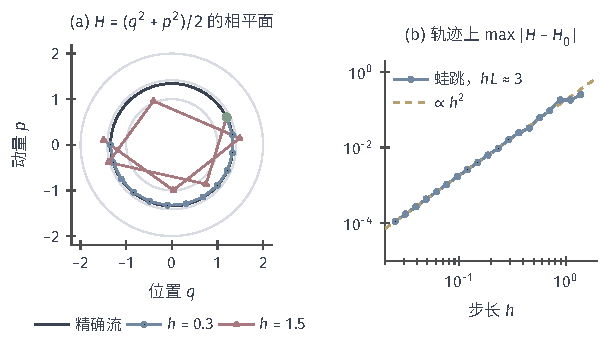
\includegraphics[width=102mm]{figures/03-optimization-evolution-and-signals/02-processes-and-trajectory-evolution/tikz/dtsp-hmc-leapfrog/figure.pdf}
  \caption{蛙跳积分的轨迹与能量误差。Hamilton量$H=(q^2+p^2)/2$，初值$(q,p)=(1.2,0.6)$（绿点）。(a)灰色为等能量圆，黑线为精确流，蓝线为$h=0.3$的$12$个蛙跳步，红线为$h=1.5$的$6$个蛙跳步；(b)总时间$hL\approx3$的轨迹上最大能量误差随步长的变化（双对数坐标），黄色虚线斜率为$2$。}
  \label{fig:dtsp-hmc-leapfrog}
\end{figure}

能量误差由Metropolis接受步校正。下面的定理对任意保体积的可微对合成立，蛙跳只是其中一例。

\begin{theorem}[对合提议的细致平衡]
  \label{thm:dtsp-hmc-balance}
  设$T$是相空间上可微、保体积的对合。以概率$\alpha(\bm z)=\min\{1,e^{H(\bm z)-H(T\bm z)}\}$从$\bm z$移到$T\bm z$、否则停在$\bm z$，所得核关于$\rho$满足细致平衡。
\end{theorem}

\begin{proof}
接受部分的密度流量为$\rho(\bm z)\alpha(\bm z)\propto\min\{\rho(\bm z),\rho(T\bm z)\}$。对任意有界可测$g$，作变量替换$\bm y=T\bm z$，由$T^2=I$及Jacobian绝对值为$1$，
\[
  \int g(\bm z,T\bm z)\min\{\rho(\bm z),\rho(T\bm z)\}\,\mathrm d\bm z=\int g(T\bm y,\bm y)\min\{\rho(T\bm y),\rho(\bm y)\}\,\mathrm d\bm y,
\]
即接受部分在交换出发点与到达点后不变。拒绝部分在对角线上，本身对称。
\end{proof}

由此得到\term{Hamilton蒙特卡洛}（Hamiltonian Monte Carlo）的一轮：保留位置$\bm q$，按$\mathcal N(\bm 0,\bm M)$重新抽取动量；从$(\bm q,\bm p)$出发走$L$个蛙跳步，翻转末端动量；以$\min\{1,e^{-\Delta H}\}$的概率接受末端位置，否则保留原位置\scite{pgm-sampling-neal2011}。动量刷新是对$\rho$的一次Gibbs更新，保持$\rho$；接受步由上面的定理保持$\rho$；二者复合仍保持$\rho$，但复合一般不再可逆。输出的位置序列按迭代编号构成一条离散时间Markov链，前面关于遍历、相关与误差评估的讨论全部适用。这里只用到确定性的常微分方程与它的离散化，不需要随机微积分。

使用时要记住它的成本与限制。每轮需要$L$次梯度计算，步长$h$决定接受率，轨迹长度$hL$决定能走多远，质量矩阵$\bm M$决定各方向的相对尺度。$U$须可微；多峰目标的峰间能量壁垒仍然难以跨越；步长若依赖当前状态，或提议不保持体积，接受率中还要加入相应的修正。Hamilton蒙特卡洛的目标是保持分布，能量并不沿轨迹下降，所以不能把它理解为一种更快的梯度下降。

\subsection{有限路径的重加权}
\label{sec:dtsp-path-reweighting}

\paragraph{整条路径的似然比}
重要性抽样也可以作用在整条路径上：手头有按一种规则生成的轨迹，想计算另一种规则下某个路径函数的平均。设$(X_0,\ldots,X_T)$在两个规律$P,Q$下关于同一参考测度分别有逐步条件密度$p_k(x_k\mid x_{<k})$与$q_k(x_k\mid x_{<k})$（$k=0$时为初始密度）。由条件密度的乘法公式，联合密度之比为
\begin{equation}
  L_T=\frac{\mathrm dQ}{\mathrm dP}(X_0,\ldots,X_T)=\prod_{k=0}^T\frac{q_k(X_k\mid X_{<k})}{p_k(X_k\mid X_{<k})},
  \label{eq:dtsp-path-likelihood-ratio}
\end{equation}
于是$\mathbb E_Q[F(X_{0:T})]=\mathbb E_P[L_TF(X_{0:T})]$。推导只用到联合分布的链式分解，不需要Markov性质。要求是：在$P$实际可能到达的每段历史上，凡$q_k>0$处都有$p_k>0$；$P$根本不会产生、而$Q$可能产生的路径，任何有限权重都无法补救。

似然比过程本身是一个鞅，这把本节与第~\ref{sec:dtsp-accumulation}节联系起来。在$P$下，
\[
  \mathbb E_P[L_{n+1}\mid\mathcal F_n]=L_n\int\frac{q_{n+1}(x\mid X_{\leq n})}{p_{n+1}(x\mid X_{\leq n})}p_{n+1}(x\mid X_{\leq n})\,\mathrm dx=L_n,
\]
最后一步用到$q_{n+1}$是概率密度且在$p_{n+1}$为零处也为零。所以$(L_n)$是均值为一的非负鞅。

\paragraph{策略轨迹的特例}
许多应用中，路径由“状态—行动”交替组成：$\tau=(s_0,a_0,s_1,a_1,\ldots,s_T)$，行动按概率核$\mu(a\mid s)$选择，下一状态按环境的转移核$P(s'\mid s,a)$产生。若要评价另一个行动规则$\pi(a\mid s)$，而初始分布与环境转移核不变，式~\eqref{eq:dtsp-path-likelihood-ratio}中环境因子在分子分母中相同而相消：
\begin{equation}
  \frac{p_\pi(\tau)}{p_\mu(\tau)}=\prod_{t=0}^{T-1}\frac{\pi(a_t\mid s_t)}{\mu(a_t\mid s_t)}.
  \label{eq:dtsp-policy-ratio}
\end{equation}
这意味着不知道环境转移概率也能计算权重。条件是$\pi(a\mid s)>0$时$\mu(a\mid s)>0$；若两种情形的环境不同，环境转移的比值必须保留。行动规则的设计与评价含义留给决策部分。

\paragraph{长路径的权重退化}
即使每一步的比值都温和，长路径的连乘也会失控。设$P$下各步增量独立服从$\mathcal N(0,1)$，$Q$下独立服从$\mathcal N(0.2,1)$，则每步对数比为$0.2x-0.02$，
\[
  \mathbb E_P[L_T^2]=\bigl(\mathbb E_Pe^{0.4X-0.04}\bigr)^T=e^{0.04T}.
\]
二阶矩随路径长度指数增长。另一方面，在$P$下$\log L_T$是均值$-0.02T$、方差$0.04T$的正态变量，所以$L_T\to0$几乎必然，而$\mathbb E_PL_T=1$始终成立：这正是第~\ref{sec:dtsp-martingale-limits}节“加倍或清零”所示的现象，期望被越来越少的路径携带。图~\ref{fig:dtsp-path-weight-degeneracy}中$N=1000$条路径的归一化有效样本比例在$T=50$时约为$0.15$，$T=200$时只剩约$0.025$，最大的一条路径一度占据总权重的三分之一以上。

\begin{figure}[htbp]
  \centering
  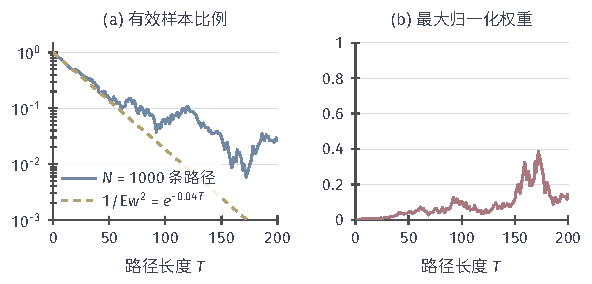
\includegraphics[width=100mm]{figures/03-optimization-evolution-and-signals/02-processes-and-trajectory-evolution/tikz/dtsp-path-weight-degeneracy/figure.pdf}
  \caption{路径权重的连乘退化。抽样规律下各步增量独立服从$\mathcal N(0,1)$，目标规律下服从$\mathcal N(0.2,1)$，$N=1000$条模拟路径（固定随机种子）。(a)归一化有效样本比例$(\sum_iL_T^{(i)})^2/(N\sum_i(L_T^{(i)})^2)$（纵轴对数刻度）与$1/\mathbb E_PL_T^2=e^{-0.04T}$；(b)最大归一化权重$\max_iL_T^{(i)}/\sum_iL_T^{(i)}$。}
  \label{fig:dtsp-path-weight-degeneracy}
\end{figure}

自归一化可以消去未知常数，却不能消除这种退化。逐步重采样把权重退化分摊到每一步，是粒子方法的核心，它与观测条件化一起属于信号与状态估计部分；连续时间路径的换测度需要额外的可积条件，在第~\ref{chap:continuous-time-stochastic-processes}章讨论。
